\documentclass[twocolumn, 10pt, a4paper]{memoir}

% standard packages
\usepackage{titlesec, blindtext, color}                                  % standard packages
\usepackage[usenames,dvipsnames,svgnames,table]{xcolor} % extra colors
\usepackage{graphicx}    
\usepackage{amsmath}                                                   % figures
%\usepackage{natbib}                                                          % bibliography
\usepackage{apacite}
\usepackage[english]{babel}
\usepackage{multirow}                                              % correct hyphenation (afbreekstreepjes)
\usepackage{booktabs}                                                     % for midrule in tables
\usepackage{array}
\usepackage{float}
\newcolumntype{P}[1]{>{\raggedright\arraybackslash}p{#1}}
\usepackage[modulo, switch]{lineno}   % use for linenumbers at the sides
% PAGE MARGINS
\usepackage[top=2.5cm, bottom=2.5cm, left=2cm, right=2cm]{geometry}

% FONT
\usepackage[lf]{berenis}
\renewcommand*\familydefault{\sfdefault}
\usepackage[T1]{fontenc}
% for other fonts, and how to install them, see the LaTeX Font Catalogue:
% http://www.tug.dk/FontCatalogue/

% LINE SPACE
\linespread{1.2}                          % more space between lines
\setlength{\parindent}{7mm}       % indenting first line paragraph
\setlength{\columnsep}{7mm} % space between columns
\linenumbers
% TABLE OF CONTENTS
% for subsubsection headers (e.g. 2.1.3), write subsubsection
% for subsection headers (e.g. 2.1), write subsection
\setsecnumdepth{subsection}        % in text
\settocdepth{subsubsection}              % in table of contents
\renewcommand{\cftdot}{}          % for no dots in table of contents
\cleardoublepage

% HYPHENATION (afbreekstreepjes)
% set words that are not abbreviated correctly (expand list when necessary)
\hyphenation{catch-ment areas a-na-lyse}

\graphicspath{ {./images/} }
%%%%%%%%%%%%%%%%%%%%%%%%%%%%%%%%%
% headers: page numbers and running titles
%%%%%%%%%%%%%%%%%%%%%%%%%%%%%%%%%

\makepagestyle{ruled}
\makeevenfoot{ruled}{}{}{}  % empty footer
\makeoddfoot{ruled}{}{}{}   % empty footer

% header left page (text on left, middle and right slot empty)
\makeevenhead{ruled}{\textcolor{gray}
	{\makebox[6mm][l]{\thepage} $|$ \hspace{3mm} \leftmark}}{}{}

% header right page  (text on right, middle and left slot empty)
\makeoddhead{ruled}{}{}{\textcolor{gray}
	{\rightmark \hspace{3mm} $|$ \makebox[6mm][r]{\thepage}}}

% first page of chapter
\titleformat{\chapter}[hang]{\vspace{-34mm}\huge}{\thechapter\hspace{20pt}\textcolor{gray}{|}\hspace{20pt}}{0pt}{\huge}
\aliaspagestyle{chapter}{chapterheader} % for no page numbers on first chapter page


%%%%%%%%%%%%%%%%%%%%%%%%%%%%%%%%%
% for background figure first page
%%%%%%%%%%%%%%%%%%%%%%%%%%%%%%%%%

\usepackage{eso-pic}
\newcommand\BackgroundPic{%
	\put(0,0){%
		\parbox[b][\paperheight]{\paperwidth}{\vfill
			\centering
			\includegraphics[width=\paperwidth,height=\paperheight,keepaspectratio]{figs/backgroundfigure.jpg}%
			\vfill
}}}



%%%%%%%%%%%%%%%%%%%%%%%%%%%%%%%%%
%%%%%%%%%%%%%%%%%%%%%%%%%%%%%%%%%
% START
%%%%%%%%%%%%%%%%%%%%%%%%%%%%%%%%%
%%%%%%%%%%%%%%%%%%%%%%%%%%%%%%%%%

\begin{document}
	
	\thispagestyle{empty}                    % otherwise it gives page number on first page
	\pagestyle{empty}
	\frontmatter
	\firmlists                                       % for less space between items in lists
	
	
	%%%%%%%%%%%%%%%%%%%%%%%%%%%%%%%%%
	% TITLE PAGE
	%%%%%%%%%%%%%%%%%%%%%%%%%%%%%%%%%
	
	%\AddToShipoutPicture*{\BackgroundPic} % for backgroundfigure
	
	
	\twocolumn[
	\begin{@twocolumnfalse}
		\begin{center}
			\vspace*{3cm}
			\fontsize{20}{20} \textbf{Improving rainfall rate estimations with Commercial Microwave Link Signals}\\
			\vspace{2cm}
			\fontsize{20}{20}\textbf{in Sri Lanka using Deep Transfer Learning}\\
			\vspace{9cm}
			\huge \textbf{Ludo Diender}\\
			\vspace{3cm}
			\large \textbf{Supervisors: Hidde Leijnse, Ruben Imhoff and Kirien Whan}\\
			\large \textbf{February 2022}\\
			\vspace{1cm}
			\large \textbf{MSc thesis}
			\large \textbf{Hydrology and Quantitative Water Management Group}\\
			\large \textbf{Wageningen University}\\
		\end{center}
	\end{@twocolumnfalse}]
	
	
	%%%%%%%%%%%%%%%%%%%%%%%%%%%%%%%%%
	% ABSTRACT
	%%%%%%%%%%%%%%%%%%%%%%%%%%%%%%%%%
	
	\cleardoublepage
	
	\twocolumn [\begin{@twocolumnfalse}
		\chapter*{Abstract}\vspace{-6mm}       % the * prevents numbering of this section
		Don't make the abstract too long. See the list of tricks on Blackbord.
	\end{@twocolumnfalse}]
	
	%%%%%%%%%%%%%%%%%%%%%%%%%%%%%%%%%
	% TABLE OF CONTENTS
	%%%%%%%%%%%%%%%%%%%%%%%%%%%%%%%%%
	
	\cleardoublepage
	% to remove table of contents name and move the text up
	%\renewcommand{\contentsname}{\vspace{-3.5cm}}
	\twocolumn[\begin{@twocolumnfalse}
		\renewcommand{\contentsname}{\vspace{-3.5cm}}
		\chapter*{Contents}\vspace{-6mm}
		\tableofcontents*
	\end{@twocolumnfalse}]
	
	
	%%%%%%%%%%%%%%%%%%%%%%%%%%%%%%%%%
	% INTRODUCTION
	%%%%%%%%%%%%%%%%%%%%%%%%%%%%%%%%%
	
	% start on right side of page
	\cleardoublepage
	
	% start with page numbering 1, 2, 3 instead of i, ii, iii
	\pagestyle{ruled}
	\mainmatter          
	
	% Chapter name
	\chapter{Introduction}\vspace{-6mm}
	\section{Context and motivation}
	
	Having ample and correct precipitation data is important for a plethora of applications, including flood warnings, agriculture, river safety and shipping routes \shortcite{Chwala2019}. In urban areas, an even higher spatial and temporal resolution of rainfall is needed, due to the complex and quickly responding urban hydrological system \shortcite{Overeem2011}. A high rain gauge density can help in providing this resolution in urban areas \shortcite{Yoon2017}, but is not always availabe. Commercial Microwave Links (CML) do typically have a high density in populated areas and could therefore help in retrieving these high-resolution urban precipitation data. CML are back-haul links used by telecommunication companies to transfer information from one telecom station to the next using microwave signals. The links' signals get attenuated by rainfall by means of scattering and absorption. The received signal level is measured and stored by the telecommunication companies for monitoring purposes and can be used to retrieve path-averaged rainfall rates by calculating the attenuation. In the past 25 years, CML have been recognized as a valuable opportunistic method to measure rainfall \shortcite{Leijnse2007, Ruf1996}. Especially in data-scarce areas, where little precipitation is measured, CML have proven to be an excellent additional information source for precipitation data \shortcite{Overeem2021,Doumounia2014,Diba2021}. Recent research has been focussing on the use of CML data to measure rainfall in tropical regions, amongst others Sri Lanka \cite{Overeem2021} and Brazil \cite{RiosGaona2017a}. Although operational use of CML signal as precipitation data source is mainly limited by the availability and accessibility of the signal data, the technique has been widely researched.
	
	The first studies on the use of CML signals to retrieve rainfall rates were done by using a specific Power Law (PL) to relate the attenuation of the signal and the rainfall rate \shortcite{Overeem2011,Leijnse2007}.Several methods have been constructed based on this PL, including RAINLINK \shortcite{Overeem2011}. The RAINLINK methodology can be described with 4 steps: 
	\begin{enumerate}
		\item wet-dry classification
		\item baseline estimation
		\item wet antenna attenuation estimation
		\item rainfall rate retrieval
	\end{enumerate}
	This method has yielded good results in multiple studies \shortcite{deVos2019,Graf2020,Fencl2017}. Recently, the community has been exploring a more data-driven approach in the form of neural networks of different architectures. Neural networks are a subpart of Machine Learning that is inspired by the neural structure of the brain. A neural network consists of different layers of nodes (neurons) that are connected to each other. If the network contains more than one layer, it is considered a deep network and Deep Learning is used as equivalent naming. A neural network is able to learn the relationship between the input and output, without intervention from a researcher. Studies have been performed in Sweden, Israel \shortcite{Habi2019}, Germany \shortcite{Polz2020}, South Korea and Ethiopia \cite{Diba2021} on the use of such data-driven networks in relating CML signals to rainfall rates. Most of these use RAINLINK or a similar method as a benchmark. Previous studies have shown that data-driven models can be more accurate, less time-demanding and more robust in estimating rainfall rates compared to the PL method \shortcite{Polz2020,Pudashine2020}.  Neural networks are not a novelty in predicting rainfall \shortcite{French1992}, but the application to CML data has recently gained popularity.
	
	\begin{figure}[t]
		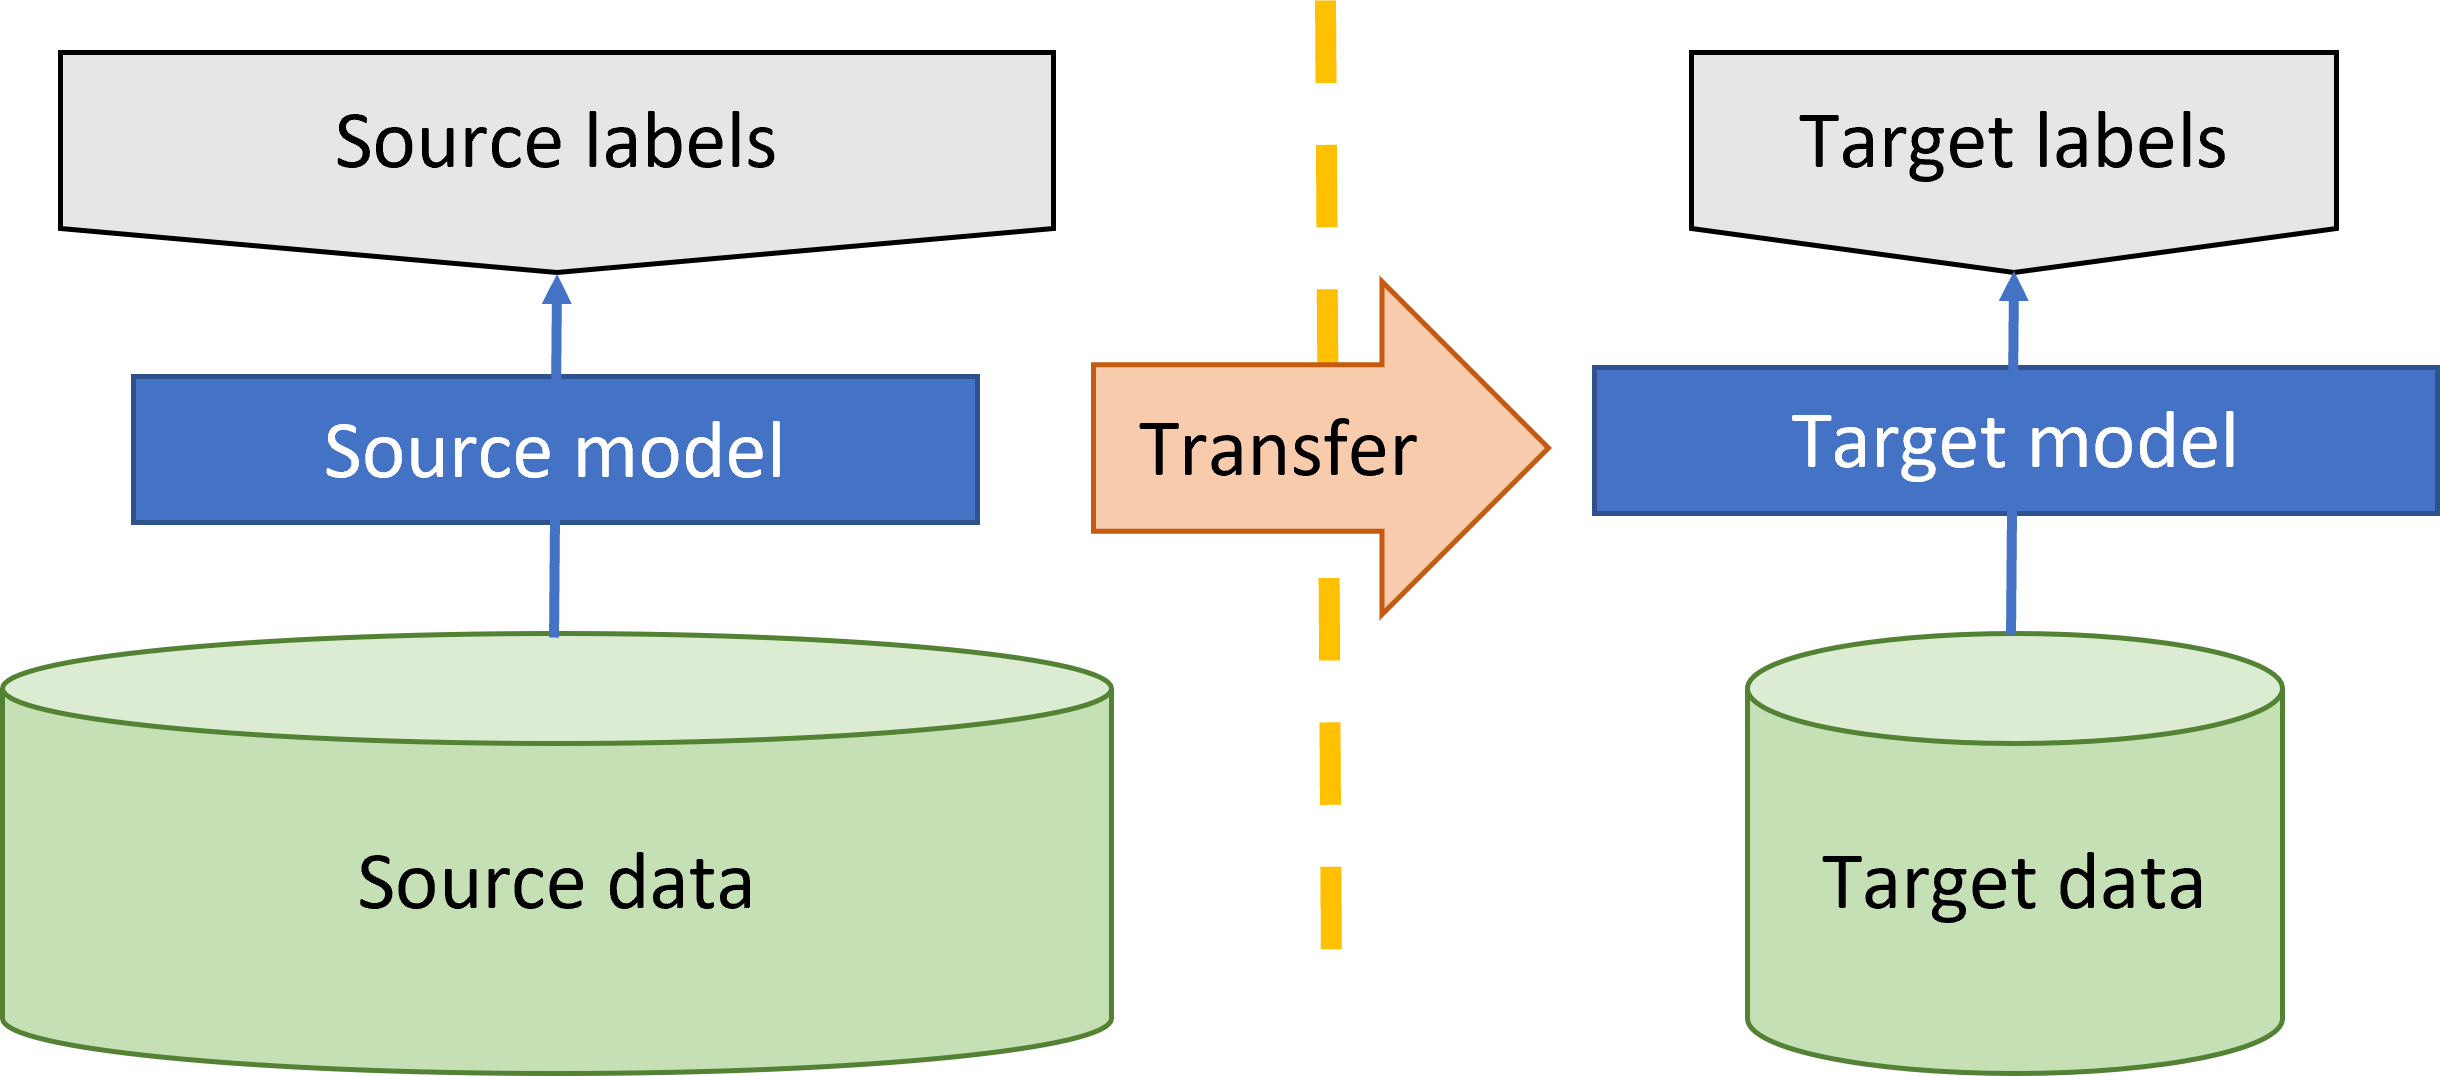
\includegraphics[width=8cm]{Transfer_learning_concept}
		\caption{Concept of transfer learning. Adapted from \protect\cite{Sarkar2018} }
		\label{fig:transferconcept}
	\end{figure}
	
	The few studies that have been performed on the combination of neural networks and CML, all focussed on a specific part of the RAINLINK methodology. \citeA{Polz2020} and \shortciteA{HabiYear} put emphasis on the wet-dry classification. \citeA{Pudashine2020} based his work around rainfall rate retrieval and Habi \citeA{Habi2019} constructed a combined model with both aspects present. All of these studies use a certain amount of preprocessing and error filtering, aside from the deep learning, to deal with the other aspects of the original PL algorithm.
	
	In focussing on a specific part of this method, the models can get more and more elaborate and complicated. Neural networks or deep learning can be a very versatile and powerful tool, but it comes at the expense of understandibility. The models can be tuned very specifically to the goal of the study, but it takes more and more time to understand the reasoning behind the final modelling output. An overarching, less complex and inclusive effort to model all steps of the RAINLINK algorithm at once has not been performed yet. This study aims to make use of the power of neural networks to deal with multiple steps in the RAINLINK algorithm at once. A deep learning effort to take all these steps into account has not yet been performed to the best of my knowledge.  
	
	
	\section{Research questions}
	This study focusses on two main research questions.
	1) How does a Neural Network perform on estimating rainfall rates from Dutch Commercial Microwave Link data by replacing all steps at once of the RAINLINK algorithm?
	2) What model (hyper)parameters have the largest influence on this performance?
	By answering these questions, this study will give a first impression of the raw power of neural networks in combination with CML signals. It gives insight in what the most important factors are to take into account. 
	
	
	\section{Thesis contents}
	This thesis starts with a description of the data that is used (Section~\ref{ch: field}). In Section~\ref{ch: methods} the methodology of this study is described. This includes an explanation on Neural Networks, data preprocessing, transfer learning and the set-up of this model study. Afterwards, in Section~\ref{ch: results} the results are presented. These results and the approach used in this study are discussed in Section~\ref{ch: discussion}, which is followed by the conclusion in Section~\ref{ch: conclusion}.
	
	
	
	
	
	
	%%%%%%%%%%%%
	% FIELD SITE AND DATA
	%%%%%%%%%%%%
	 
	\cleardoublepage
	\chapter{Data}\vspace{-6mm}\label{ch: field}
	In this study, two types of data are used: Commercial Microwave Link (CML) signal data which is used as input to the model, and precipitation observations (gauge-adjusted radar) as reference to evaluate the model. Both types of data will be elaborated upon in this section.
	
	
	\section{Commercial Microwave Link} \label{sec: CML data}
	The CML data used in this research is the same as used in previous research \shortcite{Overeem2016}.
	The CML data is received from NOKIA microwave links, operated by T-Mobile. The dataset spans from January 14 2011 until June 30 2013. The dataset consists of  3101 links, but as shown before \shortcite{Overeem2016}, not all of these links are useful or continuously available. The total number of actual links used will therefore be lower, depending on the availability of the data. On average, around 2500 links are used at a time. THe minimum and maximum Received Signal Level (RSL) in decibel-milliwatts (dBm) is stored at 15-minute intervals. The power resolution of this data is 1 dB. 
	
	\begin{figure}[h]
		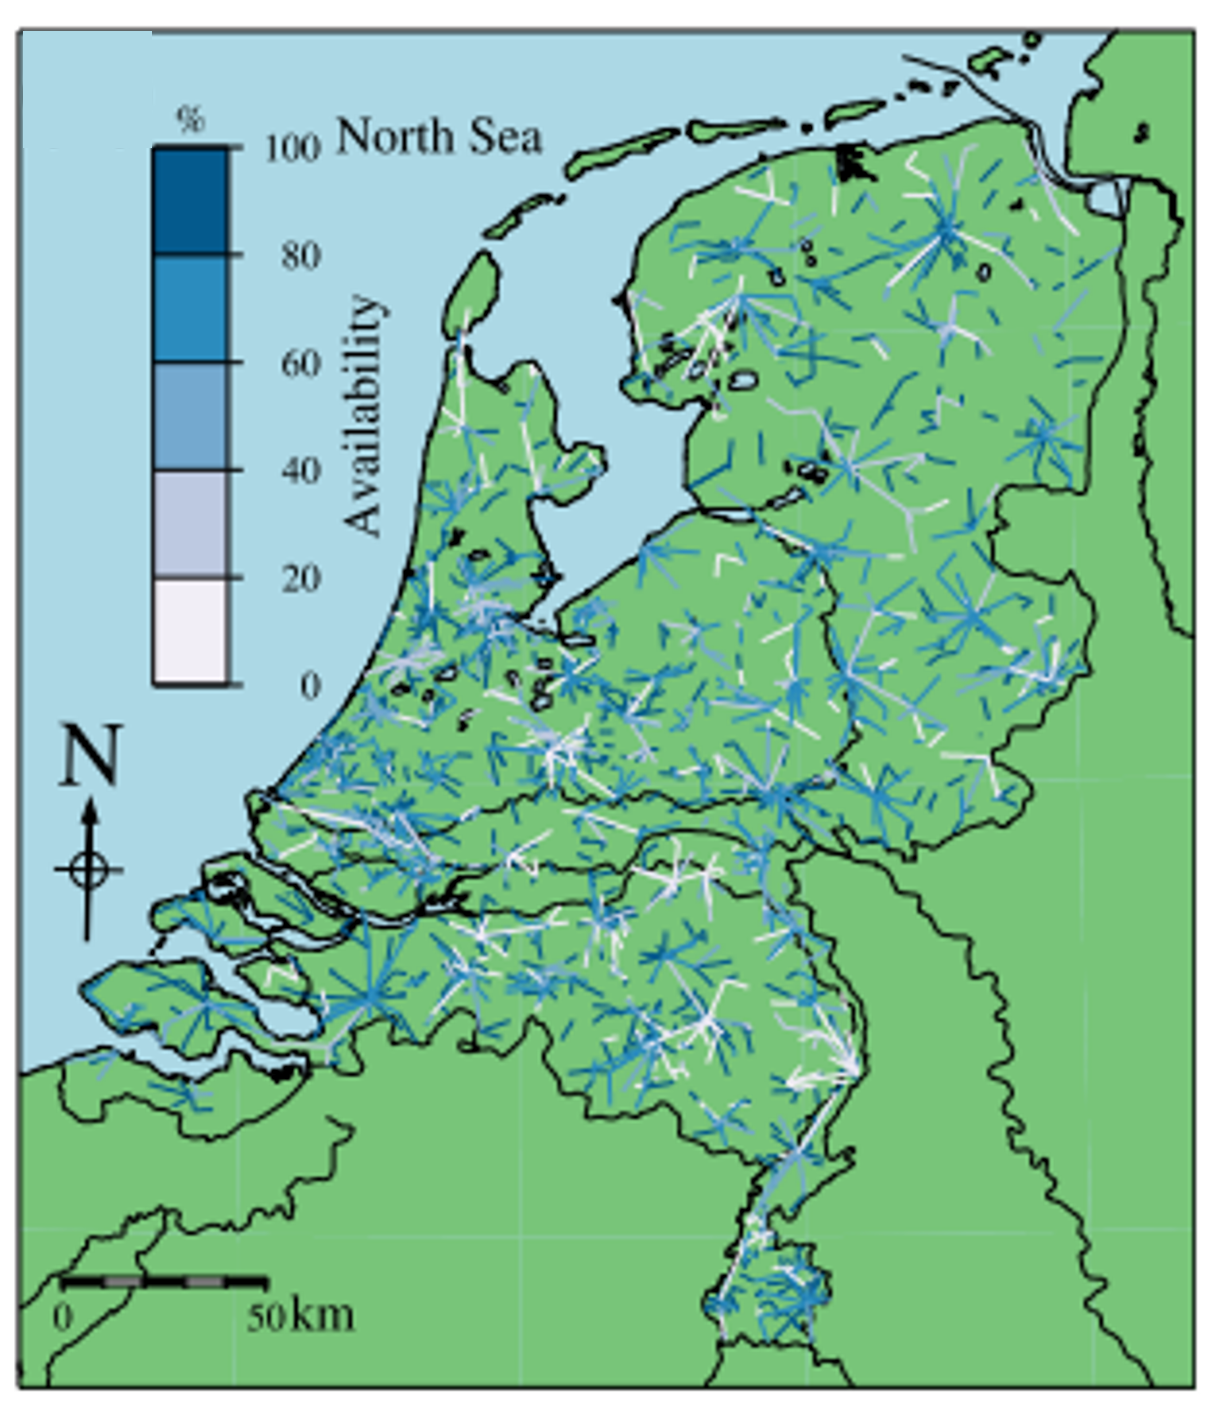
\includegraphics[height= 9cm]{Dutch_CML_network}
		\caption{Used CML network in the Netherlands. Retrieved from \protect\citeA{Overeem2016}}
		\label{fig: cmlnetworkmaps}	
	\end{figure}


	\begin{figure}[h]
		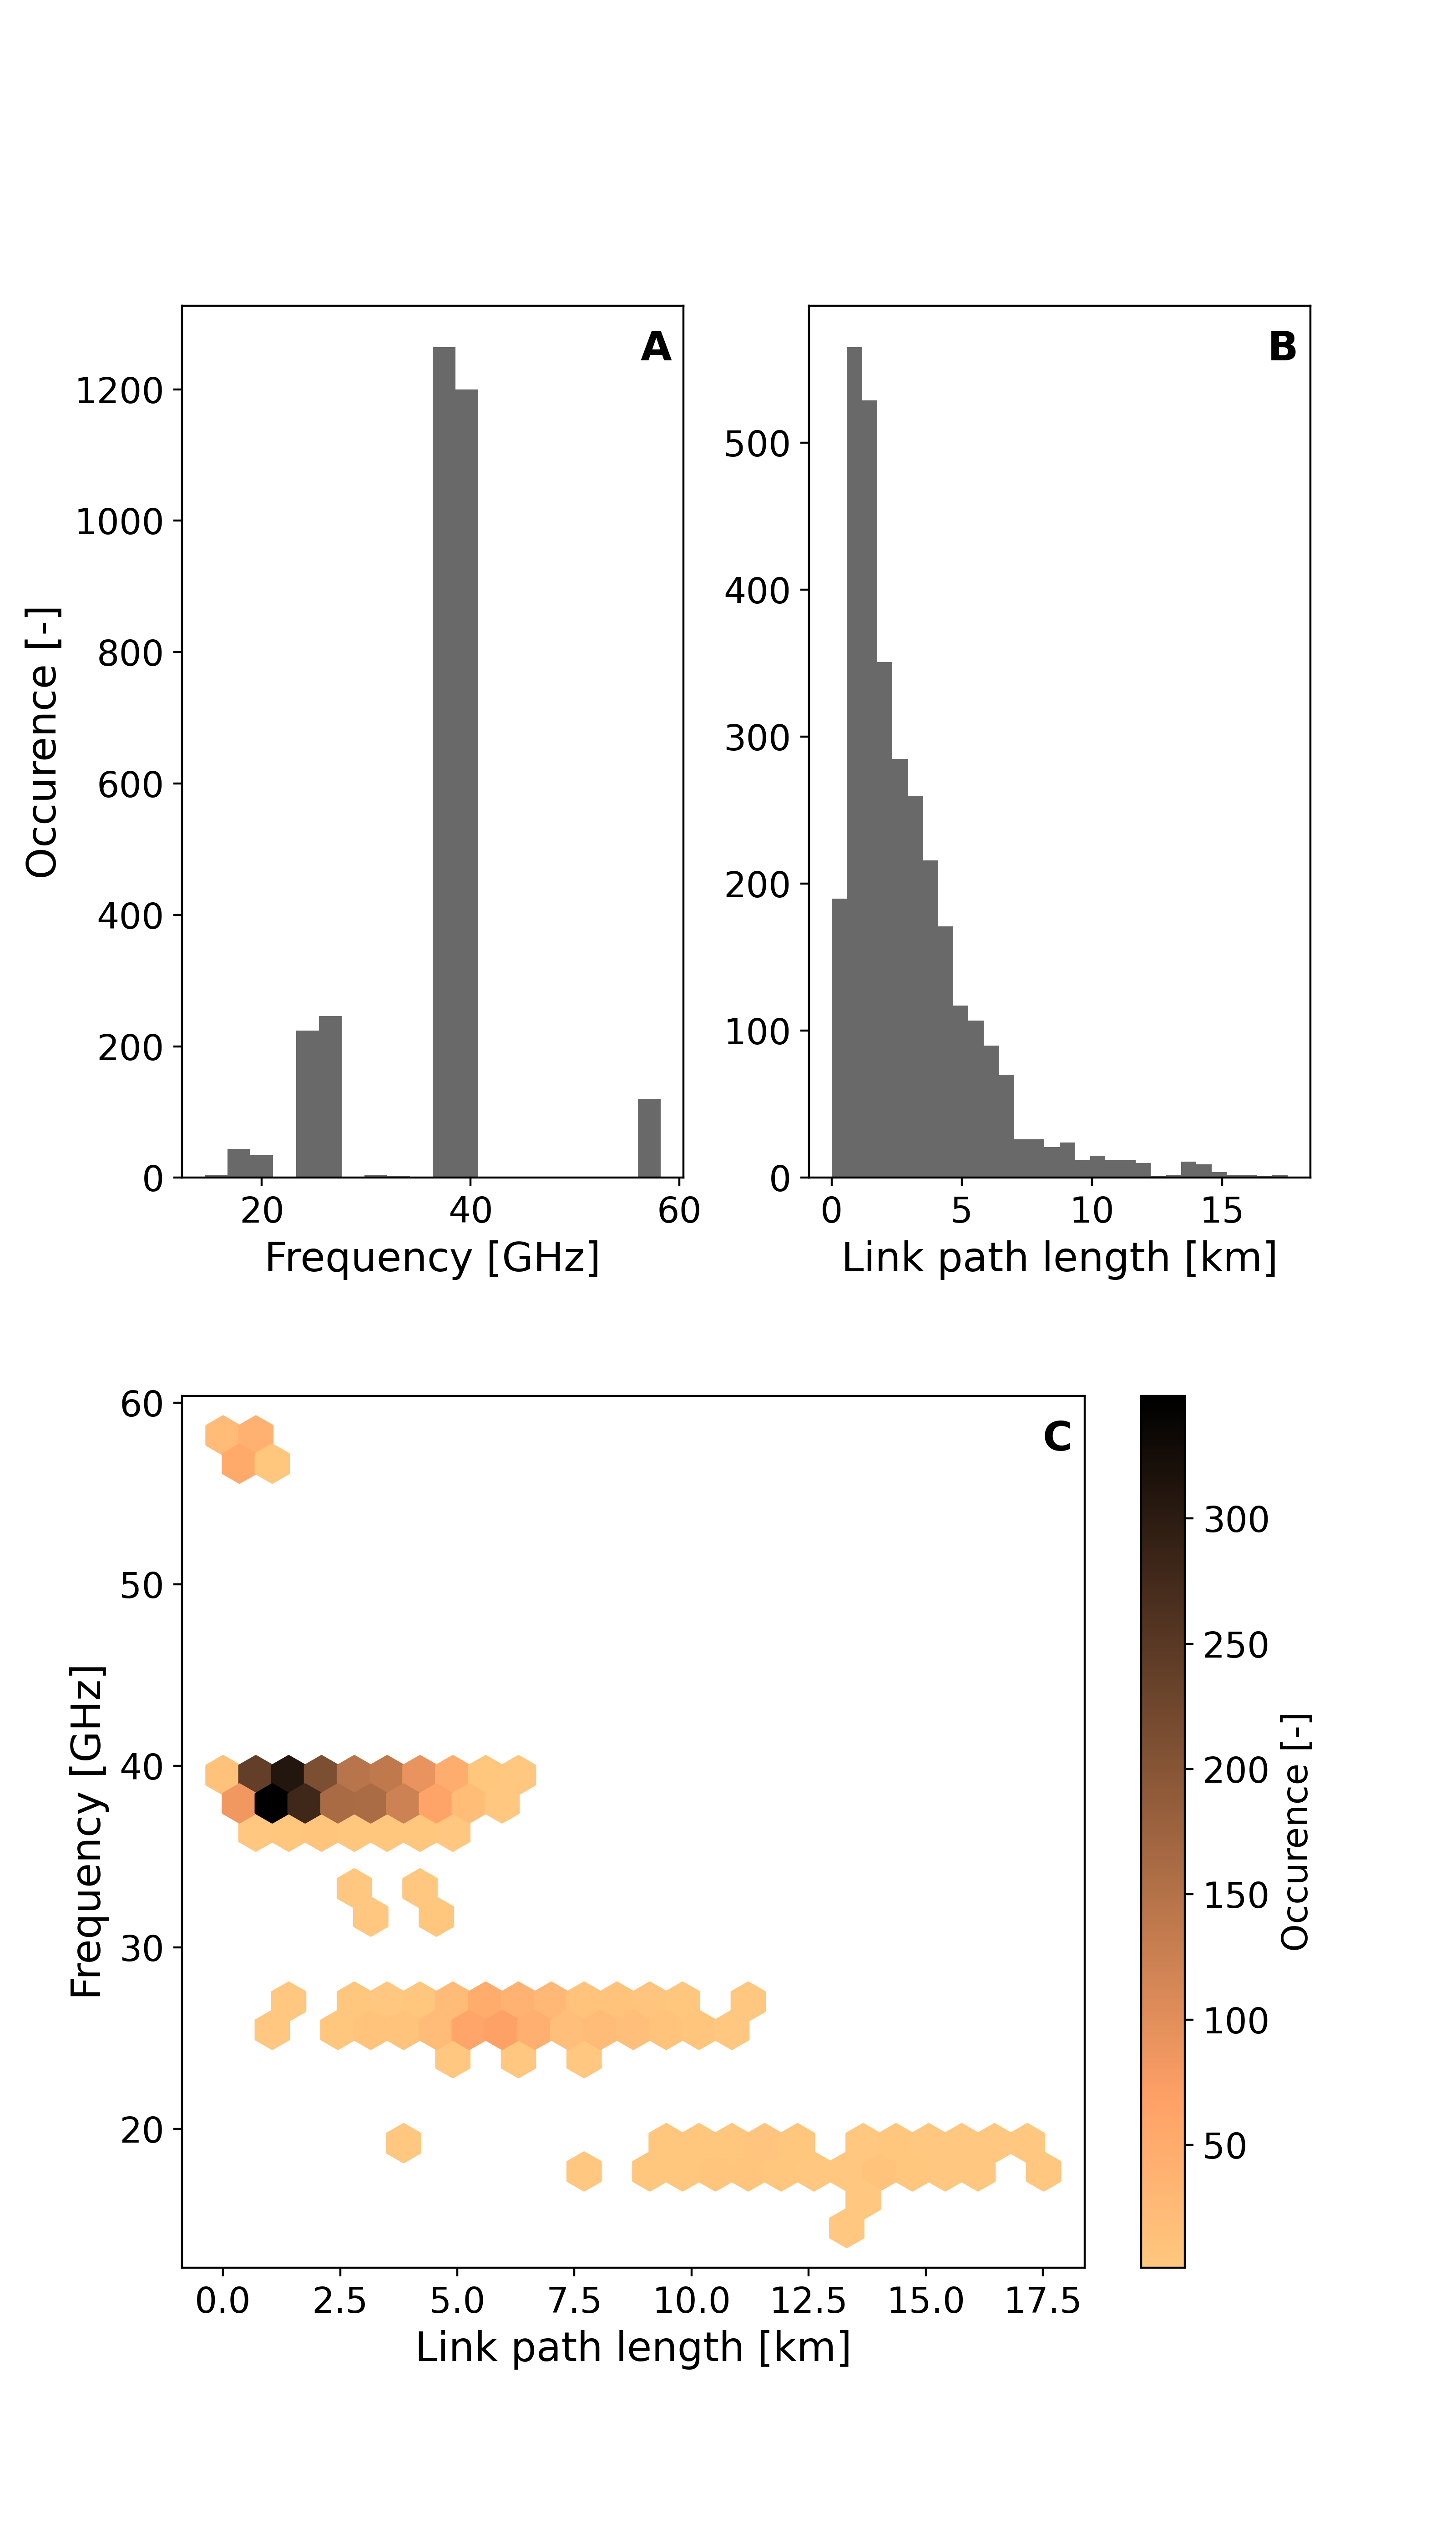
\includegraphics[width=10cm]{val_freq_dist}
		\caption{Static data for the CMLs with a) the frequency distribution, b) the link path length distribution and c) the occurence of the combination of the two parameters. Figures apply to the final independent test set covering half of 2013 (see Section~\ref{sec: datasplitting})}
		\label{fig: CML validation}
	\end{figure}

	Apart from the dynamic time signal data, static metadata is included as well. This includes coordinates of the start and end point of the link, distance between these points and frequency per link. Figure \ref{fig: cmlnetworkmaps} shows the distribution of the links throughout the Netherlands, where the highest link density can be found around urban areas. The frequency at which the links operates and the distance the links cover determine the baseline for the link's signal, which is the second step in the RAINLINK methodology. Their respective distributions can be found in Figure~\ref{fig: CML validation} a and b. Figure~\ref{fig: CML validation} c shows the combined distribution of the distance and frequency. The spikes in the frequency distributions indicate that the links roughly operate at 4 different frequencies. The distance distributions shows that although most links operate at quite short distances (<4 km), there are still links included in the data set that cover over 5 or even 10 km. The effects of link path length and frequency on the estimation of precipitation has been discussed before by \citeA{Leijnse2008}.	
	
	
	

	
	\section{Gauge-adjusted radar precipitation} \label{sec: Ref prec data}
	The precipitation observations are taken from the gauge-adjusted radar rainfall product\footnote{Freely available as "Radar precipitation climatology" via http://climate4impact.eu} with a resolution of 1 km\textsuperscript{2}. The radarmeasurements are adjusted with the use of both automated and manual rain gauge networks operated by the Royal Netherlands Meteorological Institute (KNMI). The gauge-adjusted radar observations are available at a 5-min temporal resolution. To match the 15-min intervals from the CML data, the precipitation data is summed to 15-min intervals. This dataset is of high quality and fully available in the considered time period (Jan 2011 - June 2013). Other studies that used the same gauge-adjusted radar data in combination with CMLs include \shortciteA{Overeem2016} and \shortciteA{Imhoff2020}.

	
	%%%%%%
	% METHODS
	%%%%%%
	
	\chapter{Methods} \label{ch: methods}
	This chapter describes the methodology of this study. The chapter starts with a general explanation on neural networks and their functioning, to get acquainted with terms and parameters in Section \ref{sec: NN explain}. Section~\ref{sec: datapreprocess} deals with the preprocessing of the input data to the model and subsequently model selection is described in Section~\ref{modelselection}. Which model runs and how their results are evaluated will be treated in Section~\ref{sec: EvalStats}. The final part of this chapter deals with transfer learning and how this is applied in this study (Section~\ref{transferlearning})
	\section{Neural network explanation} \label{sec: NN explain}
	\subsection{Goal and concepts of neural networks} \label{sec: NNConcepts}
	Neural networks are a subset of models within the Machine Learning (ML) environment. All models within the ML space are data-driven, i.e. without pre-specified relationships between input and output. These data-driven models aim to figure out this relationship via self-learning techniques.
	The biggest advantages of such models are that 1) they are very versatile: they can adapt to various circumstances and can be used in a wide range of applications, and 2) they can learn relationships that we do not have a physical explanation for yet. Through multiple iterations, the models can improve by minimizing or maximizing a loss function. The loss function can be interpreted as a score for the model: the worse the score, the more the model needs to adjust itself (see Section~\ref{sec: Learning NN}).It improves by optimizing parameters of differential equations in the model. Similar to physically-based models, it is up to the modeler to determine when the model performs well enough. The self-learning ML models will stop learning after a certain criterion is met, or when a specified number of iterations has passed.
	
	Neural networks are inspired by the structure of the human brain with neurons and synapses, hence the name neural network. The network consists of one or multiple layers of nodes that are connected with each other. When the network has more than one layer, it is called a deep neural network and it is referred to as Deep Learning. Every single connection between nodes (or between nodes and input/output) is represented by a weight and a bias. These weights and biases are the bread and butter of neural networks. They determine the underlying relationships between different parts of the input signal, the connections within the model and the relation to the final output. Training a neural network is all about adjusting the weights and biases in such a way that the desired output is created. At every node, a weighted sum is calculated based on these weights and biases and it is passed to an activation function. This activation function yields one value, which will be passed to the following nodes in the model.
	Because of the very general structure of neural networks, they form a very versatile set of models. Research efforts in neural networks span from image classification and speech recognition to time series prediction and weather forecasts.
	
	\subsection{Neural network architectures} \label{sec: NN architecture}
	The versatility of neural networks allows for a wide range of different model architectures to choose from. Every architecture has its own strengths and weaknesses. For image recognition for example, the most common type of neural network is a convolutional neural network (CNN). In time series prediction, the most common architecture is the recurrent neural network (RNN), which is therefore most suited for precipitation estimation using Commercial Microwave Links.
	
	RNNs are looping-based architectures, which make them ideal for dealing with sequences. The core unit of RNNs, the Recurrent Unit (the lightgreen blocks in Figure \ref{fig: multilayer RNN}), is used multiple times. The output of the unit is added to the input of the next step in the same recurrent unit. This creates an architecture that is well suited for time series with sequential data patterns. How many layers of these recurrent units are used in a model depends on the modeler and can be tuned (see Section \ref{sec: modelselection})
	
	One of the limitations of default RNNs is the lack of memory in the model. Information from the start of a sequence is quickly lost throughout the model. A Long Short Term Memory (LSTM) model circumvents this problem by having an extra stream of information. This stream of information carries aspects of the previous time steps and can be viewed as a 'memory highway'. Every layer of the network has a separate memory stream which carries information from the start of the sequence. At every LSTM cell, information is taken from the memory state as input to the cell, and an adapted memory state is given as output. Most cells in an LSTM model have three input streams: the memory state, the new input state and the hidden output state from the previous time step. Within each cell, the three input streams are used to produce three output states as well: the updated memory state, a hidden output for the next cell in the sequence and a hidden output for the next layer in the model. The conversion from these three inputs to three outputs is where the weights and biases come into play in an LSTM model. As an LSTM cell is a recurrent cell as well, there is one cell with weights and biases per layer of the network. Information is recurrently added to this cell. A schematic representation of the model used in this study can be found in figure~\ref{fig: multilayer RNN}.
	
	After the information has passed through all LSTM layers of the model, the final hidden outputs are fed into the fully connected or dense layer (see figure~\ref{fig: multilayer RNN}). This layer takes the intermediate output from the LSTM cells and connects them to the desired output of the model. The dense layers outputs a sequence of values, the same length as the input sequence. In this study, a many-to-one architecture is used. This means that a sequence of signal levels is used to predict one rainfall rate at a specific timestep. Referring to figure~\ref{fig: multilayer RNN}, only the rightmost output ($O_n$) is considered the output of this model.
	
	For more information on the internal functioning of LSTM cells, a more in depth explanation of their power and their evolution to their current shape and form, the reader is refered to \citeA{Staudemeyer2019}.
	The LSTM approach in this study is similar, although not identical, to \citeA{Habi2019}. 
	
	\begin{figure*}
		\center
		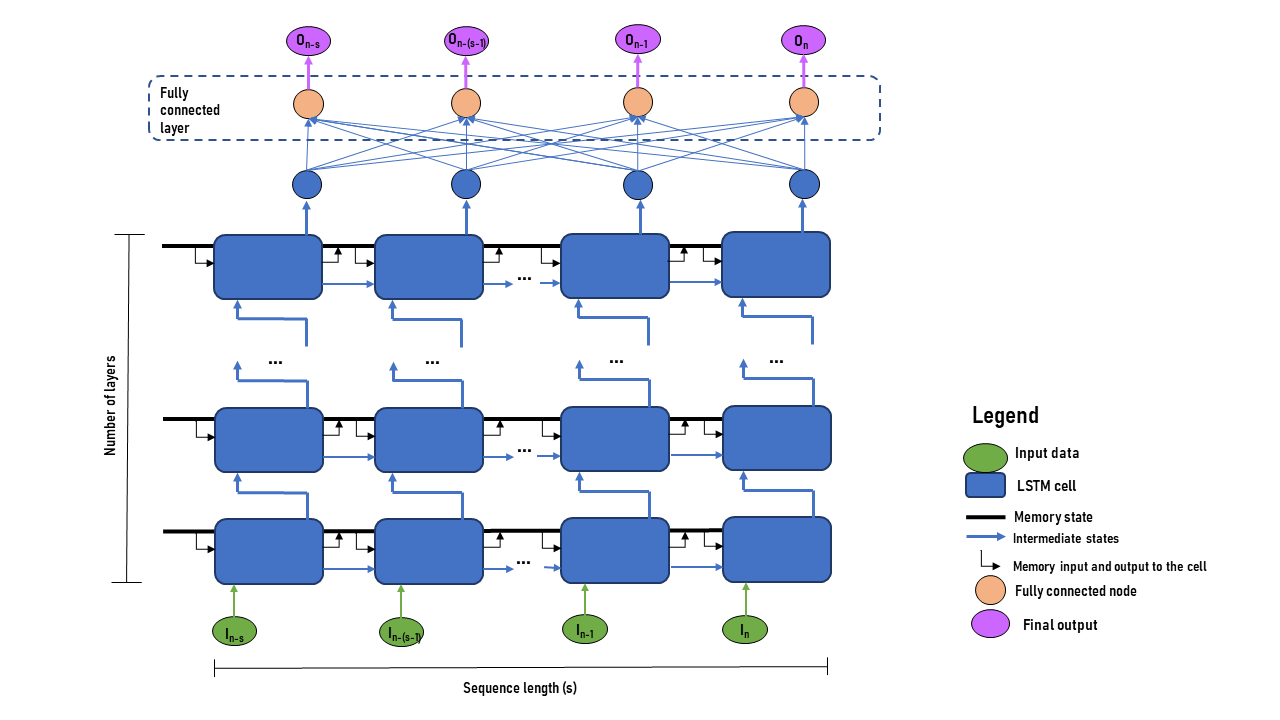
\includegraphics[width=\textwidth]{C:/Users/ludod/Documents/GitHub/Thesis_HWM2021/Thesis/images/Schematic_LSTM_TR_23_3_LudoDiender.png}
		\caption{\textit{Schematic representation of a two-layer unfolded RNN. HS represents the hidden state,X is the input, O is the output and U, V and W are weight and bias vectors associated with the model}}
		\label{fig: multilayer RNN}
	\end{figure*}
	
	\subsection{Learning process of neural networks} \label{sec: Learning NN}
	The self-learning ability of neural networks is mainly relying on the loss function. The model calculates the error between its output and the target output and tries to adjust accordingly. The selected loss function determines amongst others the behavior of the model. In this study, a standard Mean Square Error (MSE) loss function is used as a basis (see Eq.~\ref{eq: MSE}).
	\begin{equation} \label{eq: MSE}
		MSE = \frac{1}{n} \sum_{i=1}^{n} (y_i - \hat{y})^2
	\end{equation}
	where ${y_i}$ is the predicted 15-min interval precipitation and $\hat{y}$ is the observed 15-min interval precipitation.
	MSE as a loss function has been used before in similar studies \cite{Pudashine2020, Diba2021}. These studies, however, had a more elaborate preprocessing of the data to correct for the inherently skewed nature of precipitation distributions. \citeA{Habi2019} showed that the loss function can also be altered to correct for this skewedness by using a Rain Distribution Factor (RDF). In this research, the application of an RDF serves two purposes:
	
	\begin{itemize}
		\item Penalize negative predictions more to force the model into predictions bigger than or equal to zero. A random initialization can cause negative output which is physically impossible.
		\item Penalize the model more for higher target variables. This steers the model towards a better prediction of the actual precipitation events.
	\end{itemize}
	\vspace{3mm}
	The RDF is defined in Eq~\ref{eq: RDF},
	\begin{equation}
		\label{eq: RDF}
		RDF=\begin{cases}
			3, & y_i < 0\\
			1-y_s e^{y_r\cdot{}\hat{y}}, & \text{otherwise}.
		\end{cases}
	\end{equation}
	where $y_i$ is the predicted rainfall rate, $\hat{y}$ is the observed rainfall rate and $y_s$ and $y_r$ are hyperparameters, set to $0.95$ and $-5$ respectively in accordance with \citeA{Habi2019}.
	
	The combination of Eq~\ref{eq: MSE} and Eq~\ref{eq: RDF} leads to the final loss function used in this thesis (Eq~\ref{eq: final_loss})
	
	\begin{equation}
		\label{eq: final_loss}
		Loss = \frac{1}{n} \sum_{i=1}^{n} RDF \ (y_i - \hat{y})^2
	\end{equation}
	
	To update and improve the model prediction, an optimizer (or propagation algorithm) is selected. Such an optimizer is a mathematical set of equations that determines how the model learns. In this study, the Adaptive Moment (ADAM) optimizer will be used. ADAM is one of the more recently introduced optimizers and has been shown to outperform other optimizations methods. \cite{Kingma2014} In simple terms: the method is looking for an optimum (minimum or maximum) per weight. Based on this gradient, the weight is adjusted up or down to minimize the loss function. As calculating the full gradient field for all weights present in the model is a tedious task, ADAM is stochastic method, which means it takes a randomly selected subset of the data and uses that to calculate the gradients. This might lead to more steps, but the steps are less computationally intensive and typically lead to an improved performance.  
	The ADAM optimizer is back-propagated. This implies that the final layer of the network is updated first and the learning process works itself back to the start of the model. In this study, the fully connected layer at the end of the LSTM is updated first before the model improves and adjusts the LSTM cells itself. A back-propagated model is chosen in this study since it is the most common type of neural network, easy to implement, fast, flexible and generally good \cite{Staudemeyer2019}.
	
	\subsection{Available hyperparameters} \label{sec: Avail hyper}
	The versatility of neural networks is generally perceived as one of the biggest advantages of these type of models. However, it does leave the modeller with a lot of options to choose from in creating a neural network for their specific task. The parameters that refer to the architecture and set-up of the neural network are called hyperparameters. Table~\ref{tab: hyperparamtable} highlights the available hyperparameters in this model. The hyperparameters will, for the purpose of this thesis, be divided in three groups: Structure, Data and Effiency. Structure hyperparameters relate to the structure of the model: how is it designed and how often will it run. Data parameters are related to the input data into the model; the type of data and the goal with the data determine these hyperparameters. The Efficiency group entails hyperparameters that relate to the time it takes the model to run. In this group, there's always a balance between performance and computational intensity. It should be noted that in the end, all hyperparameters influence the computational speed of the model in some way or another. The proposed grouping is not strict but rather serves the purpose of dealing with hyperparameters with a specific function in a structured way.
	
	\begin{table*}[ht]
		\caption{Available hyperparameters in this study.}
		\hspace*{\fill}
		\label{tab: hyperparamtable}
		\centering
		\renewcommand{\arraystretch}{1.5}
		\begin{tabular}{P{0.8cm}P{2.0cm}P{12.8cm}}
			\hline
			Group&Hyperparameter&Description\\
			\hline
			\multirow{4}{*}[-35pt]{\rotatebox{90}{Structure}}&Hidden size&Size of the intermediate hidden output. Higher hidden size allows for more complex relations\\
			&Learning rate&A multiplication factor that influences the speed at which the weights in the model are updated with each SGD step. A high learning rate makes the model learn faster, but also makes it more prone to overfitting.\\
			&Number of epochs&The number of iterations the model performs to reach the final prediction. More epochs improve the performance of the model but take sginificantly longer to run.\\
			&Number of layers&Total number of layers in the model. A higher number of layers creates a model that can better identify complex dependencies in the data.\\
			\midrule
			\multirow{2}{*}[-14pt]{\rotatebox{90}{Data}}&Sequence length&Length of datasample used to predict one target value.\\
			&Loss function&Metric that is used to judge the model performance on. Can be tailored towards the goal of the model.\\
			\midrule
			\multirow{4}{*}[-15pt]{\rotatebox{90}{Efficiency}}
			&Batch size&The size of each batch of data that is fed to the model. The larger the batch size, the faster the model will be able to learn, but the less possiblities it has to update its weights and biases.\\
			&Optimizer&The algorithm that is used to update the weights and biases of the model internally.\\
			&Scheduler&The algorithm that is used to run multiple combinations of hyperparameters simultaneously and decides when early stopping of trials is necessary\\
			
			\bottomrule
			
		\end{tabular}
		\hspace*{\fill}
	\end{table*}
	
	The process of calibrating hyperparameters in order to find an optimal combination (if it exists) is refered to as tuning. Not all hyperparameters were automatically tuned. Only the Structure hyperparameters were tuned, as the other two hyperparameter groups need to be determined based on the input data and the available computational resources. More details on the automatically tuned Structure hyperparameters can be found in Section \ref{sec: RayTune}. The Data and Efficiency group of hyperparameters are set based on convenience and literature study and will be elaborated on in Section \ref{sec: Nonauto tuning}.
	
	
	\section{Data preprocessing} \label{sec: datapreprocess}
	\subsection{Connecting CML and reference data}
	To train the model, a feature set (received signal levels) and a target set (precipitation observations) is needed. For every separate CML link and every time step, the corresponding amount of precipitation has been determined. To obtain this value, the middle point of each link has been determined and connected to the corresponding radar cell. This midpoint method is commonly used in CML research (refs). More elaborate methods have been used by \shortciteA{Leijnse2007} for example, where a weighted sum of all cells that the link passes through was created. The impact of this decision will be discussed further on in this thesis.
	\subsection{Error filtering}
	A large part of the RAINLINK algorithm consists of error filtering. Because the algorithm cannot distinguish a signal distortion by rain or by a bird, this filtering is necessary. The spirit of Deep Learning models is that these errors don't need to be filtered out manually. Similar to Habi et al., just the 'no data' values have been removed from the dataset. The model is expected to handle other noise in the data by learning the patterns and adjust accordingly.
	\subsection{Data splitting and scaling}
	A Deep Learning model with a varying set of hyperparameters needs three independent datasets to run: a training set, a validation set and a test set.The training dataset is used to improve the models weights and parameters and is fed through the SGD algorithm, in which the model is updated in a backwards propagating fashion. The validation set is subsequently used to independently judge the performance of the model. This set needs to be as independent as possible, to prevent overfitting of the model.
	As different models with different combinations of hyperparameters are tested, a third independent test set is needed to check how well the best model out of these different combinations performs.  
	
	In creating the three separate datasets, multiple approaches can be taken. The core of the split is based on the IID principle (Independent and Identically Distributed) \cite{Hampel1998}:
	
	\begin{itemize}
		\item There is little to no information leaked from one set to the other (truly independent datasets)
		\item There is enough data in each of the sets to cover a wide range of events and situations (comparable datasets and thus assumed identically distributed)
	\end{itemize}
	IID data ideally does not have any internal dependencies in the data left that could complicate the model's ability to generalize. 
	
	The data for the Netherlands has been split in a 40/40/20 for training, validating and testing respectively. Previous studies use varying ratios to split the data, with the one common aspect being a smaller validation set compared to the training and testing \cite{Polz2020,Diba2021,Pudashine2020}. This particular split has been chosen as a rough average of these varying ratios.
	The year 2011 is used for training, 2012 for testing and 2013 (up until July 21st) for validating. By taking full years for training and testing, all seasons are incorporated and the datasets are assumed to be closer to being identically distributed. Considerations on and implications of this split will be discussed later on in this thesis in section \ref{sec: datasplitting}
	
	Having large outliers and ranges in the input data can cause the Adam algorithm to have exploding gradients. Therefore, a scaling has been applied to both the features and targets. 
	The targets (precipitation observations) have been scaled using a inverse hyperbolic sine transformation, which is a variant on the more common log transformation \cite{Kilmartin1972}. To deal with zero values, which are ominous in precipitation data, and to handle extreme values better, Burbidge \citeA{Burbidge1988} introduced the inverse hyperbolic sine transformation. This transformation is defined as in Eq~\ref{eq: logsine}.
	
	\begin{equation}
		\label{eq: logsine}
		y_t = \log(y_i + \sqrt{y_i^2 + 1})
	\end{equation}
	where $y_t$ is the transformed variable and $y_i$ is the raw variable.
	Afterwards, the logsine-transformed precipitation data were scaled with the minimum and maximum per dataset, to create a value between 0 and 1. As three separate datasets were used, this implies three slightly different scalings. As the goal is to minimize information leakage from one dataset to the next, this separated scaling is preferred, in order to not further violate the aforementioned IID assumption.
	
	The features (RSL) have been scaled differently. As the base level of each CML is dependent on the frequency and the distance of the link, the median of each link has been subtracted from the signal. Subsequently, the data has been divided by the standard deviation per dataset to obtain values that are closer to eachother. By subtracting the median of each link from the signal, a very crude form of baseline estimation has been applied (step 3 in the RAINLINK methodology). As data needs to be rescaled anyways in order to avoid exploding or vanishing gradients, this specific scaling has been included in the methodology of this study. 
	
	
	
	\section{Model selection} \label{sec: modelselection}
	This section deals with selecting the right model structure for the study at hand. It is worth noting that there might be multiple combinations of hyperparameters that lead to the same results (a variant on the concept of equifinality). In section~\ref{sec: Equifinality} this concept will be elaborated on and the impact on the followed procedure will be discussed.
	
	\subsection{Automated hyperparameter tuning} \label{sec: RayTune}
	A full grid search on all hyperparameters available to find the best combination is computationally infeasible. Therefore, this study uses 25 random combinations of hyperparameters, all within a limited range of values. This number of combinations is chosen to have a trade-off between computational intensity and having ample combinations to ensure a decent search.
	Selecting the combinations is done using the RayTune package, which is a tuning-specific Python package that interacts with PyTorch (used in this study) and other Deep Learning packages. This study uses the Async Successive Halving Algorithm Scheduler (ASHA) to effectively search the hyperparameter space. The ASHA Scheduler is able to effectively implement parallelism (to decrease runtime) and a hard early stopping mechanism to terminate runs if they are not amongst the best few models after a while \cite{Li2018}. The ASHA Scheduler is the most common scheduler available in RayTune and performs well in most cases when no specific instructions regarding hyperparameter tuning are needed.  
	The best combination of hyperparameters is used to calculate the model performance based on the final independent testset. The ranges for the calibrated hyperparameters can be found in Table~\ref{tab: raytunetable}
	
	\begin{table}
		\caption{Ranges for the automatically tuned hyperparameters using RayTune.}
		\label{tab: raytunetable}
		\centering
		\renewcommand{\arraystretch}{1.5}
		\begin{tabular}{P{2.5cm}P{4.2cm}}
			\hline
			$Hyperparameter$&$Range$\\
			\hline
			Hidden size&$[8,32,64,128,256]$\\
			Learning rate&$1e^{-6} - 1e^{-3}$\\
			Number of epochs&$(10 - 50)$\\
			Number of layers&$[2,4,8,16]$\\
			\hline
		\end{tabular}
	\end{table}
	
	\subsection{Non-automated hyperparameter tuning} \label{sec: Nonauto tuning}
	Hyperparameters that are related to the data rather than the model itself are not tuned automatically. Hyperparameters in the Data group are tuned, but in a slightly less rigid way as it is easier to deduct which values should perform well on the input data.
	The sequence length is partly determined by how long rainfall events typically last in the Netherlands and their autocorrelation. As a starting value, a sequence length of 8 (15-min) timesteps is used. This means that the past two hours are used to predict the rainfall rate at the current time step. A sequence length of one hour (4 timesteps) and three hours (12 timesteps) will be evaluated as well to inspect the impact of a different sequence length.
	The loss function has a direct relation to the distribution of the input data. The chosen loss function (\ref{eq: final_loss} should be able to deal with the skewedness of the data. To check if this is the case and whether the extra effort of including a RDF is worth it, a normal MSE loss function (\ref{eq: MSE} will be tested as well.
	
	From the Efficiency group, the batch size is the most important hyperparameter to evaluate.\citeA{Kandel2020} described the effect of the batch size on the final performance of the model. The batch size and the learning rate are intimately linked: a smaller batch size requires a lower learning rate and vice versa. A batch size of 32 is used as standard, but the options of batch sizes of 64 and 128 are explored as well. A batch size of 32 has been shown to be a good default value \cite{Bengio2012}. Using a power of 2 as batch size is common to fully use GPU processing power.
	
	\section{Experimental setup and evaluation of results} \label{sec: EvalStats}
	For this study, different model runs are performed. In the first run, all automatically tuned hyperparameters mentioned in Section~\ref{sec: RayTune} are included. The 25 different randomly chosen model runs, as picked by the random selector in RayTune, are depicted in Table~\ref{tab: hyperparameter combi}. 
	
	\begin{table}[t]
		\label{tab: hyperparameter combi}
		\caption{Different hyperparameter combinations used for the tuning experiment.}
		\hspace*{\fill}
		\centering
		\renewcommand{\arraystretch}{1.2}
		\begin{tabular}{P{0.4cm}P{1.2cm}P{1.2cm}P{1.4cm}P{1.2cm}}
			\toprule
			\multicolumn{1}{c}{Model ID} & Hidden size & Learning rate & Number of epochs & Number of layers \\ \midrule
			1                            & x           & x             & x                & x                \\
			2                            & xx          & x             & x                & x                \\
			3                            & x           & x             & x                & x                \\ 
			4                            & x           & x             & x                & x                \\
			5                            & x           & x             & x                & x                \\
			6                            & x           & x             & x                & x                \\
			7                            & x           & x             & x                & x                \\
			8                            & x           & x             & x                & x                \\
			9                            & x           & x             & x                & x                \\
			10                           & x           & x             & x                & x                \\
			11                           & x           & x             & x                & x                \\
			12                           & x           & x             & x                & x                \\
			13                           & x           & x             & x                & x                \\
			14                           & x           & x             & x                & x                \\
			15                           & x           & x             & x                & x                \\
			16                           & x           & x             & x                & x                \\
			17                           & x           & x             & x                & x                \\
			18                           & x           & x             & x                & x                \\
			19                           & x           & x             & x                & x                \\
			20                           & x           & x             & x                & x                \\
			21                           & x           & x             & x                & x                \\
			22                           & x           & x             & x                & x                \\
			23                           & x           & x             & x                & x                \\
			24                           & x           & x             & x                & x                \\
			25                           & x           & x             & x                & x                
		\end{tabular}
		
	\end{table}
	The model run with the best score on the independent test set will be used to test different non-automatically tuned hyperparameter settings. This results in three more combinations of model runs, where the batch size, the loss function and the sequence length are evaluated respectively with their ranges as put in Section~\ref{sec: Nonauto tuning}.
	For the final model run, only timesteps that show precipitation are taken into account. This functions as a very crude wet-dry classification, the first step in the RAINLINK methodology. By running the model only on rain samples, we investigate the impact of using such a wet-dry classification, as multiple previous studies included a model part on this step \cite{Habi2019}.

	The model results will be evaluated using the coefficient of determination (R$^{2}$, see Eq~\ref{eq: R2}), the Coefficient of Variation (CV, Eq~\ref{eq: CV}) and the Root Mean Square Error (RMSE, Eq~\ref{eq: RMSE}).
	\begin{equation} \label{eq: R2}
		R^2 = 1- \frac{\sum_{i=1}^{N} (\hat{y}_i - y_i)^2}{\sum_{i=1}^{N} (y_i - \bar{\hat{y_i}})^2}
	\end{equation}

	\begin{equation} \label{eq: CV}
		CV = \frac{\sigma}{\bar{y}}
	\end{equation}

	\begin{equation} \label{eq: RMSE}
		RMSE = \sqrt{\frac{1}{n} \sum_{i=1}^{n} (y_i - \hat{y_i})^2}
	\end{equation}
	where $y_i$ is the predicted 15-min precipitation rate, $\hat{y_i}$ is the observed 15-min precipitation rate and $\sigma$ is the standard deviation of the predicted 15-min precipitation rate.
	These statistical evaluation metrics will be able to tell something about the fit of the model prediction to the observed values. The selected metrics are based on similar studies that use these metrics to evaluate their model performance \shortcite{Overeem2011, Pudashine2020,Diba2021}.
	
	%%%%%%
	% RESULTS
	%%%%%%
	
	\chapter{Results} \label{ch: results}
	Figure~\ref{fig: loss epochs} shows the validation loss for the 25 different combinations of hyperparameters. Due to the random initialization of each model, the starting losses differ between the runs. Almost all combinations show a decreasing loss over the epochs, which indicates the self-learning capabilities of the neural network. Some models hardly improve over time or even worsen. This particuliar behaviour could be caused by the overfitting of the model on the training dataset. The best model yields a final loss of [INSERT RDF MSE LOSS HERE].
	
	\begin{figure}[h]
		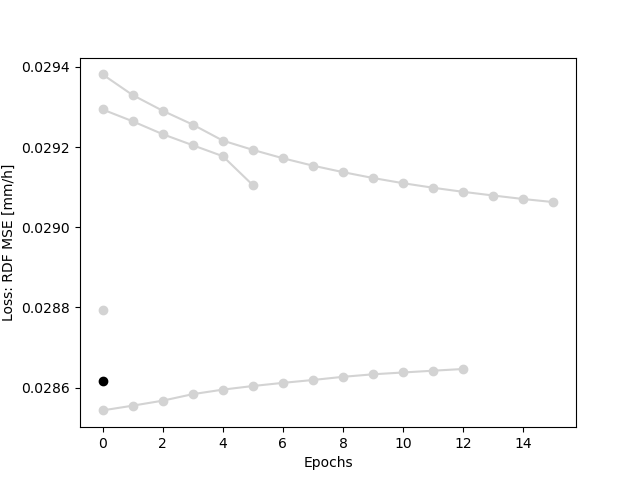
\includegraphics[width=\columnwidth]{ex_loss_epochs}
		\caption{The validation loss (RDF MSE) per epoch for all 25 tuning runs. The best model that will be used for subsequent model runs is depicted in black.}
		\label{fig: loss epochs}
	\end{figure}

	The performance of the best combination of hyperparameters on the final independent test set is depicted in figure~\ref{fig: scatter statistics}. This shows that the model, although it improved over time, manages to predict one specific value the majority of the time. The observed range in precipitation rates and the modelled range in precipitation rates are vastly different. The range of the prediction is orders of magnitude smaller than the observed range. The CV of [INSERT CV] and RMSE of [INSERT RMSE] do not tell the complete story of the prediction, as their values are in line with previous research \cite{Pudashine2020}. The R\textsuperscript{2} of [INSERT R2] however does indicate the poorness of the modelled fit. The investigated hyperparameters for these runs are not the deciding factors in this modelling effort and the predictions and observations are still widely different. The impact of other hyperparameters and the exclusive use of samples with a precipitation rate above 0 will be showed in the following figures. 
	
	
	\begin{figure}
		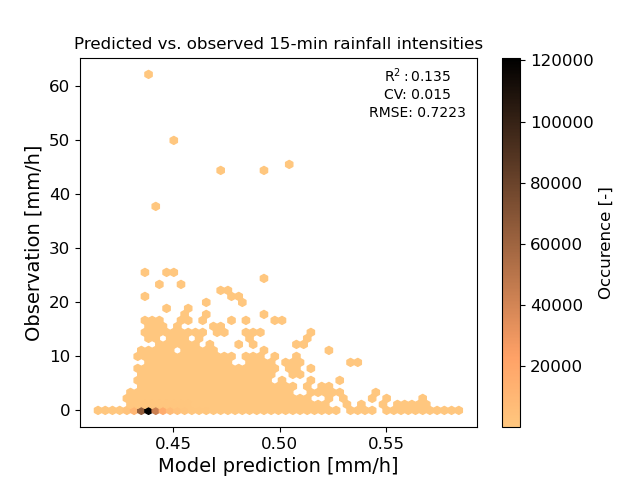
\includegraphics[width=\columnwidth]{scatter_final}
		\caption{Predicted versus observed precipitation for the best model configuration out of Figure~\ref{fig: loss epochs}.}
		\label{fig: scatter statistics}
	\end{figure}
	Summarizing table with statistics on RAINLINK vs My Model
	

	
	\chapter{Discussion} \label{ch: discussion}
	The discussion of this research will be split up in two parts. The first parts deals with the more general assumptions and choices that have been made in this modelling effort and their implications, consequences and impacts, supported by previous studies. The second part, the outlook, deals with the very poor results of this study. This part describes what possible shortcomings of this methodology could be, what could be included in future similar modelling efforts to improve the results and finally some recommendations for follow up investigations on this topic. 
	\section{Assumptions and choices}
	\subsection{Data splitting} \label{sec: datasplitting}
	The chosen years are not identical in their precipitation distributions. The year 2011 was somewhat drier than average, with a particularly dry spring. 2012 was slightly wetter than average, with above average precipitation in the first and last month of the year. Finally, 2013 had a dry winter with some snow and a very wet autumn, yielding a yearly average precipitation considerably lower than average. \cite{KNMI}  
	This inconsistency in precipitation over the years violates the IID assumption that underpins the datasplit. It highlights the tradeoff that has been made in creating this split. Ideally, all datasets would have an equal identical precipitation distribution. However, wherever two datasets meet in time, there is a chance of information leaking from one dataset to the other. If the years would have been reshuffled to create a more identically distributed split, there would have been more information leaking from one set to the other and the independence of the datasets would have been at stake. Therefore, this split by full years was still preferred, to minimize information leakage. For the test set, half a year is taken due to limitations in data availability. As the validation set is only used to judge the final model, and not to update the model anymore, this dataset can be smaller as for example in \citeA{Pudashine2020}.
	
	Due to the aforementioned reasons, the data is not perfectly IID. Apart from the more abstract discussion whether the IID principle is ever really attainable (as there are always some long term dependencies in your data according to \citeA{Hampel1998}), the impact of not having precisely IID data has been discussed before. Several studies have dealt with data that is not IID. \shortciteA{Lin2016} proposed a method where the non-IID data is further split up in small groups that can be assumed to be IID. The loss per group is determined and the maximum average loss per group was taken as a loss function. \citeA{2019} suggested a numerical algorithm to solve this method for non-linear problems.
	
	Although the data is not perfectly IID, during this study we deemed it non necessary to implement a specific algorithm suitable for non-IID data. Both training and validation data include all 4 seasons, have a full year span and have not been filtered on any sort of events. When the model would be evaluated with a completely new independent dataset, this dataset could also include the natural variability that is present in these datasets. As the sets are long enough, the effect of not perfectly IID data is assumed to not have a major influence on the final results. Studies that used similar data before used a similar split of the data, assuming that this split guarantees the data to be sufficiently IID \cite{Diba2021,Pudashine2020}.
	
	
	\subsection{Equifinality and optimal hyperparameter combination} \label{sec: Equifinality}
	Trying out different types of NN and different hyperparameters: thousands to choose from
	
	\subsection{No signal picked up} \label{sec: no results}
	More preprocessing of the data: stronger error filtering, only including the wet events (so wet-dry classficiation). Separate models with separate architectures for the different parts of the algorithm: a classifying CNN for the wet/dry, LSTM for baseline estimation, normal ANN for WAA and another LSTM for the final rainfall retrieval.
	
	\section{Outlook}
	Wat is de manier verder vanaf hier: wat zou wel kunnen werken? 
	Including more information like neighbouring links
	%%%%%%%%%%%%
	% CONCLUSION
	%%%%%%%%%%%%
	
	\chapter{Conclusion} \label{ch: conclusion}
	Does my model outperform RAINLINK in the NL?
	DL models have potential but there is a lot a lot to customize
	
	%%%%%%%%%%%%%%%%%%%%%%%%%%%%%%%%%
	% ACKNOWLEDGEMENTS
	%%%%%%%%%%%%%%%%%%%%%%%%%%%%%%%%%
	
	
	\chapter*{Acknowledgements}\vspace{-6mm}       % the * prevents numbering of this section
	\addcontentsline{toc}{chapter}{Acknowledgements}   % to get acknowledgements in table of contents
	
	Don't forget to thank the people who gave you data!
	T-Mobile Ralph Koppelaar \& Ronald Kloeg 
	Aart Overeem
	%%%%%%%%%%%%%%%%%%%%%%%%%%%%%%%%%
	% BIBLIOGRAPHY
	%%%%%%%%%%%%%%%%%%%%%%%%%%%%%%%%%
	
	\renewcommand{\bibname}{Bibliography}
	\bibliographystyle{myapacite}
	\bibliography{Thesis_Ludo}
	
	% to add items to the bibliography:
	% option 1. open "references_thesis.bib" in JabRef (free downloadable), enter more papers
	% option 2. open "references_thesis.bib" in NotePad, go to Google Scholar, find paper, click "cite", click "import into BiBTeX", copy text into NotePad
	
	
	%%%%%%%%%%%%%%%%%%%%%%%%%%%%%%%%%
	% APPENDIX
	%%%%%%%%%%%%%%%%%%%%%%%%%%%%%%%%%
	
	\appendix
	\chapter{Additional figures}
	
	
	%%%%%%%%%%%%%%%%%%%%%%%%%%%%%%%%%
	% END
	%%%%%%%%%%%%%%%%%%%%%%%%%%%%%%%%%
	
	
\end{document}